\documentclass[]{beamer}

% beamer options
	%\setbeamercovered{transparent}
% custom commands
	\def\colorize<#1>{%
\temporal<#1>{\color{red!50}}{\color{black}}{\color{black!50}}}

\usepackage{tikz}
\usetikzlibrary{arrows, shapes.geometric, backgrounds}
\usepackage{minted}

\author{Tejas Sanap}
\title{Introduction to \LaTeX}
\date{December 28, 2019}

\begin{document}
	\begin{frame}
		\titlepage
	\end{frame}

	\begin{frame}[fragile,t]
		\frametitle{How do we write a document?}
			The process of creating a document comprises of two components:
			\onslide<1->{
				\begin{itemize}
					\item Deciding \textbf{what} the content \textbf{should be}\ldots
					\item Deciding \textbf{how} the content \textbf{should look}\ldots
				\end{itemize}
			}
			\onslide<2>{
				\begin{figure}
					\centering
					\def\cirA{}
					\def\cirB{}
					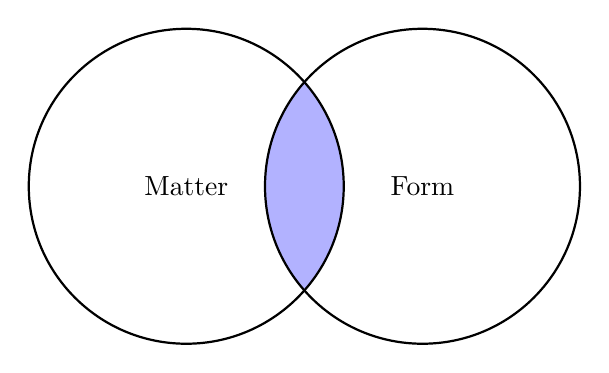
\begin{tikzpicture}[thick, fill=blue!30]
						\scope 
							\clip (0,0) circle (2cm);
							\fill (3,0) circle (2cm);
						\endscope
						\draw (0,0) circle (2cm) node {Matter};
						\draw (3,0) circle (2cm) node {Form};
					\end{tikzpicture}
				\end{figure}
			}
	\end{frame}

	\begin{frame}[t]
		\frametitle{Type-setting?}
		\onslide<1->{What is type-setting?}

		\onslide<2->{
		\begin{itemize}
			\item The process of arranging the various objects on a page.
			\item It is process that takes place after the manuscript has been written.
		\end{itemize}
		}
		\only<3-4>{
			How \only<3>{do}\only<4>{should} we typeset? \\
			\only<3>{\Huge{MS WORD!}}
			\only<4>{\Huge{{\LaTeX}!}}
		}
	\end{frame}

	\begin{frame}
		\frametitle{Why do I need \LaTeX?}
		\onslide<1->{ To save time and efforts. }
		\begin{itemize}
			\item<2-> \LaTeX does all the type-setting for you.
			\item<3-> It also auto-generates:
				\begin{itemize}
					\colorize<3> \item Table of content
					\colorize<4> \item List of figures and tables
					\colorize<5> \item Captions
					\colorize<6> \item Headers and footers
					\colorize<7> \item Page numbers (both roman and decimal)
				\end{itemize}
		\end{itemize}
	\end{frame}

	\begin{frame}
		\frametitle{What is \LaTeX?}
		\begin{itemize}
			\item A type-setting system.
			\item An improvement over \TeX.
			\item Not a WYSIWYG editor.
			\item Uses simple plaintext.
			\item \LaTeX provides the user with a set of pre-defined templates.
		\end{itemize}
	\end{frame}

	\begin{frame}
		\frametitle{How do I use \LaTeX?}
		\only<1-2>{
		\tikzstyle{block} = [rectangle, draw=red, dashed, thick]
		\tikzstyle{arrow} = [thick, ->, >=stealth]
		\tikzstyle{arrow1} = [thick, ->, >=stealth, draw=red]
		\begin{tikzpicture}{node=2cm}
			\onslide<1>{\node (texfile) [] {\texttt{.tex}};}
			\onslide<2>{\node (texfile) [block] {\texttt{.tex}};}

			\node (pdfengine) [right of=texfile, xshift=3cm] {\texttt{xelatex}};
			\onslide<1>{\node (xeengine) [above of=pdfengine, yshift=2cm] {\texttt{pdftex}};}
			\onslide<2>{\node (xeengine) [block, above of=pdfengine, yshift=2cm] {\texttt{pdftex}};}
			\node (luaengine) [below of=pdfengine, yshift=-2cm] {\texttt{lualatex}};
			\onslide<1>{\node (pdffile) [right of=pdfengine, xshift=3cm] {\texttt{.pdf}};}
			\onslide<2>{\node (pdffile) [block, right of=pdfengine, xshift=3cm] {\texttt{.pdf}};}
			\node (psfile) [above of=pdffile, yshift=2cm] {\texttt{.ps}};
			\node (dvifile) [below of=pdffile, yshift=-2cm] {\texttt{.dvi}};

			\node (source) [below of=texfile, yshift=-3cm] {\textbf{Source Code}};
			\node (source) [below of=pdfengine, yshift=-3cm] {\LaTeX\,\textbf{engine}};
			\node (source) [below of=pdffile, yshift=-3cm] {\textbf{Final Output}};

			\draw [arrow] (texfile) -- (pdfengine);
			\onslide<1>{\draw [arrow] (texfile) -- (xeengine);}
			\onslide<2>{\draw [arrow1] (texfile) -- (xeengine);}
			\draw [arrow] (texfile) -- (luaengine);
			\draw [arrow] (pdfengine) -- (pdffile);
			\draw [arrow] (pdfengine) -- (psfile);
			\draw [arrow] (pdfengine) -- (dvifile);
			\onslide<1>{\draw [arrow] (xeengine) -- (pdffile);}
			\onslide<2>{\draw [arrow1] (xeengine) -- (pdffile);}
			\draw [arrow] (xeengine) -- (psfile);
			\draw [arrow] (xeengine) -- (dvifile);
			\draw [arrow] (luaengine) -- (pdffile);
			\draw [arrow] (luaengine) -- (psfile);
			\draw [arrow] (luaengine) -- (dvifile);
		\end{tikzpicture}
		}
		\only<3> {
			There are multiple \TeX engines:
			\begin{itemize}
				\item{\textbf{Knuth's} \TeX}: \\
					This is original \TeX engine which serves as the lowest layer of \LaTeX's software architecture.
				\item{\texttt{pdftex}}: \\
					This engine adds a bunch of primitives related to the PDF and DVI extension.
				\item{\texttt{xetex}}: \\
					This engine provides better font support.
				\item{\texttt{luatex}}: \\
					Originally, meant to replace \texttt{pdftex}, but, now moving in a very different direction. This engine also better font support (like, \texttt{xelatex}) through Lua code.
			\end{itemize}
		}
	\end{frame}

	\begin{frame}[fragile]
		\frametitle{Structure of {\LaTeX} source file.}
		\begin{minted}[beameroverlays, linenos, autogobble]{latex}
			\documentclass{article}

			\usepackage{hyperref}

			\title{A critical analysis of Naruto: the Manga}
			\author{Tejas Sanap}

			\begin{document}
				\maketitle
				
			\end{document}
		\end{minted}
	\end{frame}

	\begin{frame}[t]
		\frametitle{Page Geometry}
		\begin{columns}
			\column{0.5\textwidth}
				\begin{enumerate}
					\item[4.] \mintinline{latex}{\topmargin}
					\item [7.] \mintinline{latex}{\textheight}
					\item[8.] \mintinline{latex}{\textwidth}
					\item[11.] \mintinline{latex}{\footskip}
				\end{enumerate}
			\column{0.5\textwidth}
			\includegraphics[width=\textwidth, height=\textheight, keepaspectratio]{images/Latex_layout.png}
		\end{columns}
	\end{frame}

	\begin{frame}[fragile]
		\frametitle{Environments}
		\visible<1-> {
		\emph{Environments} are used to format a bunch of text in {\LaTeX} documents instead of doing it in only one place. }
		\vfill
		\begin{visibleenv}<2->
			Example:

			\begin{minted}[beameroverlays, linenos, autogobble]{latex}
				\begin{center}
					The Jinchuriki.
				\end{center}
			\end{minted}
		\end{visibleenv}
		\vfill
		\begin{visibleenv}<3>
			A few of the most common environments we see are:

			\begin{itemize}
				\item \texttt{align}.
				\item \texttt{figure}.
				\item \texttt{equation}.
				\item \texttt{document}.
			\end{itemize}
		\end{visibleenv}
	\end{frame}
\end{document}
